\documentclass{beamer}

\setlength{\leftmargini}{1em}
\setbeamertemplate{itemize item}[circle]
\setbeamertemplate{frametitle}
{
\raggedright\insertframetitle%
}

\usepackage{lipsum}

\usepackage{agda}
\usepackage{apacite}
\usepackage{catchfilebetweentags}
\usepackage{changepage}
\usepackage{babel}
\usepackage{bookmark}

\usepackage{graphicx}

\usepackage[autostyle=true,french=guillemets,maxlevel=3]{csquotes}

\graphicspath{ {images/} }

\usepackage{newunicodechar}
\newunicodechar{∋}{$\ni$}
% \newunicodechar{·}{$\cdot$}
\newunicodechar{⊢}{$\vdash$}
\newunicodechar{≔}{$\Rightarrow$}
\newunicodechar{⋆}{${}^\star$}
\newunicodechar{Π}{$\Pi$}
\newunicodechar{⇒}{$\Rightarrow$}
\newunicodechar{ƛ}{$\lambdabar$}
\newunicodechar{∅}{$\emptyset$}
\newunicodechar{∀}{$\forall$}
\newunicodechar{ϕ}{$\Phi$}
\newunicodechar{ψ}{$\Psi$}
\newunicodechar{ρ}{$\rho$}
\newunicodechar{α}{$\alpha$}
\newunicodechar{β}{$\beta$}
\newunicodechar{μ}{$\mu$}
\newunicodechar{σ}{$\sigma$}
\newunicodechar{≡}{$\equiv$}
\newunicodechar{Γ}{$\Gamma$}
\newunicodechar{∥}{$\parallel$}
\newunicodechar{Λ}{$\Lambda$}
\newunicodechar{₀}{$~_0$}
\newunicodechar{₁}{$~_1$}
\newunicodechar{₂}{$~_2$}
\newunicodechar{₃}{$~_3$}
\newunicodechar{θ}{$\theta$}
\newunicodechar{Θ}{$\Theta$}
\newunicodechar{∘}{$\circ$}
\newunicodechar{Δ}{$\Delta$}
\newunicodechar{λ}{$\lambda$}
\newunicodechar{⊧}{$\models$}
\newunicodechar{⊎}{$\uplus$}
\newunicodechar{η}{$\eta$}
\newunicodechar{⊥}{$\bot$}
\newunicodechar{Σ}{$\Sigma$}
\newunicodechar{ξ}{$\xi$}
\newunicodechar{ℕ}{$\mathbb{N}$}
\newunicodechar{ᵇ}{${}^b$}
\newunicodechar{ᶜ}{${}^c$}
\newunicodechar{Φ}{$\Phi$}
\newunicodechar{Ψ}{$\Psi$}
\newunicodechar{⊤}{$\top$}
\newunicodechar{≐}{$\doteq$}
\newunicodechar{≣}{$\triangleq$}
\newunicodechar{≃}{$\simeq$}
\newunicodechar{≅}{$\cong$}
\newunicodechar{≢}{$\neq$}
\newunicodechar{∙}{$\bullet$}
\newunicodechar{ℓ}{$\ell$}
\newunicodechar{ℚ}{$\Q$}
\newunicodechar{ℤ}{$\Z$}
\newunicodechar{⦃}{$\{$}
\newunicodechar{⦄}{$\}$}
\newunicodechar{≤}{$\leqslant$}
\newunicodechar{≥}{$\geqslant$}
\newunicodechar{≟}{$\doteq$}
\newunicodechar{∈}{$\in$}
\newunicodechar{↣}{$\rightarrowtail$}
% \newunicodechar{}{$$}


\newunicodechar{∣}{\ensuremath{\mathnormal{\|}}}
\newunicodechar{∷}{\ensuremath{::}}

\newcommand{\agda}[2]{\ExecuteMetaData[latex/#1.tex]{#2}}

\usetheme{Frankfurt}

\DeclareQuoteStyle{english}
  {\em}
    {\em}
    {\textquotedblleft\em}
    {\em\textquotedblright}

% Information to be included in the title page:
\title{Formalizing a crypto currency prototype \\
  using dependent types in Agda }
\author[Guilherme H. A. Silva]{Guilherme Horta Alvares da Silva}
% \institute{Fundação Getulio Vargas}
\date{2022}


\begin{document}

\frame{\titlepage}

\section{Introduction}

\begin{frame}
\frametitle{Goal}
\begin{itemize}
  \item Using Agda's dependent types to create a formal definition of a crypto currency similar to Bitcoin and Ethereum.
    
\includegraphics[width=8cm, height=5cm]{bitcoin-ethereum}
\end{itemize}
\end{frame}

\begin{frame}
   \frametitle{Definition}
\begin{itemize}[<+->]
     \item A cryptocurrency is a decentralized mean of exchange that uses
       blockchain and cryptography to create new currency units and ensure the validity of transactions.
     \item In this project, I will define cryptographic functions, transactions, block and blockchain.
     \item Distributed system aspects are outside of the scope of this work.
     \end{itemize}
\end{frame}

\AgdaHide{
\begin{code}
module main where

open import Level using (Level)
open import Data.Product
open import Data.Bool
open import Data.Nat as ℕ
open import Data.Nat.Properties
open import Data.Nat.Solver
open import Data.List hiding (sum; lookup)
open import Data.Vec
open import Data.Vec.Properties
open import Data.Unit using (⊤; tt)
open import Data.Empty
open import Data.Sum hiding (map)
open import Data.Fin hiding (_+_; _≥_; _≤_; _-_; _≟_)
open import Data.Product hiding (map)
open import Function renaming (Injective to InjectiveSetoid)
open import Relation.Binary.PropositionalEquality
open import Relation.Nullary
open import Utils

open ≡-Reasoning
\end{code}
}

\section{Crypto Functions}

\begin{frame}
  \frametitle{Bitcoin Account}
    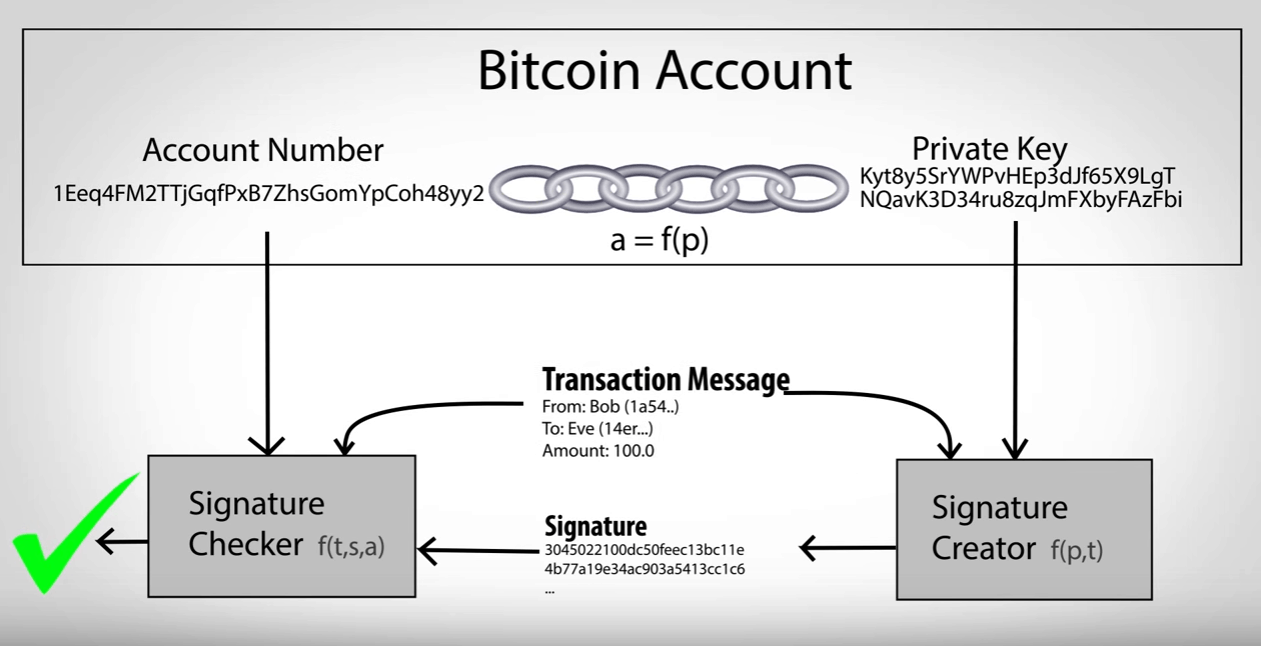
\includegraphics[width=11cm, height=7cm]{privatekey}
\end{frame}

\begin{frame}
  \frametitle{Hash Function}
  \begin{itemize}[<+->]
    \item A hash function serves to fingerprint large data into a number.
    \item It is assumed that two different files will always have different hashes (injectivity)
   since the probability of two different files having the same hash is negligible.
    \item By the pigeonhole principle, the injectivity of the hash is impossible.
      However, two files that have the same hash were never found in SHA-256.
    \item It is also not possible to compute the inverse of the hash function.
  \end{itemize}
\end{frame}

\begin{frame}
  \frametitle{Cryptographic Functions}
  \begin{itemize}[<+->]
    \item In cryptography, there is a private and a public key.
    \item From the private key, it is possible to generate a public key
 and to sign a transaction.
    \item It is not possible to know the private key from the public key and signature generated by it.
    \item It is possible to know if a signature and a public key coincide with the same private key that generates both of them.
    \item These functions are based on the SHA-256 hash function.
  \end{itemize}
\end{frame}

\AgdaHide{
\begin{code}
private variable
  ℓ : Level
  A B : Set ℓ
  MSG : Set

Injective : (A → B) → Set _
Injective = InjectiveSetoid _≡_ _≡_

_-_[_] : (m n : ℕ) (m≥n : m ≥ n) → ℕ
m - .zero [ z≤n ] = m
.(suc _) - .(suc _) [ s≤s m≥n ] = _ - _ [ m≥n ]
\end{code}
}

\begin{frame}
  \frametitle{Hashable}
\begin{code}
Hashable : Set ℓ → Set ℓ
Hashable A = A ↣ ℕ
\end{code}

\AgdaHide{
\begin{code}
instance
  open Injection hiding (cong)

  Hashableℕ : Hashable ℕ
  to Hashableℕ = id
  Injection.cong Hashableℕ refl = refl
  injective Hashableℕ refl = refl
\end{code}
}

\begin{code}
isHashFunctionℕ : (f : ℕ → ℕ) → Set
isHashFunctionℕ f = Injective f

HashFunctionℕ : Set
HashFunctionℕ = Σ[ f ∈ (ℕ → ℕ) ] isHashFunctionℕ f

module Hashableℕ
  (hashFunctionℕ@(hashℕ , _) : HashFunctionℕ) where

  hash : ⦃ Hashable A ⦄ → A → ℕ
  hash ⦃ hashA ⦄ = to hashA

  hashBoth : ⦃ Hashable A ⦄ → ⦃ Hashable B ⦄ → A → B → ℕ
  hashBoth ⦃ hashA ⦄ ⦃ hashB ⦄ a b = hash (hash a + hash b)
\end{code}


\end{frame}


\begin{frame}
  \frametitle{Crypto Constants}
\begin{code}
  record CriptoSets : Set₁ where
    field
      PrivateKey         : Set
      PublicKey          : Set
      hashablePublicKey  : Hashable PublicKey
      Signature          : Set

    instance
      _ = hashablePublicKey

    Address = ℕ
    Amount  = ℕ

    address : PublicKey → Address
    address = hash
\end{code}

\end{frame}

\begin{frame}
  \frametitle{Postulates}
  \begin{itemize}[<+->]
    \item Hash injective is impossible to proof.
      But we postulate it because the probability of hash collision is very low.
    %% hash should be Fin n
    \item In my master thesis, each function of crypto was postulated.
      However, it is better to put these functions as variables.
      Therefore, the code can be more general for every crypto function that has these properties.
  \end{itemize}
\end{frame}

\begin{frame}
  \frametitle{Postulates}
  \begin{code}
  record WithCryptoPostulates (cryptoSets : CriptoSets)
    : Set₁ where
    open CriptoSets cryptoSets public
    field
      priv→pub : PrivateKey → PublicKey
      Signed   : ⦃ Hashable MSG ⦄ → MSG
                 → PublicKey → Signature → Set
      Signed?  : ∀ ⦃ _ : Hashable MSG ⦄ (msg : MSG) pk sig
                 → Dec $ Signed msg pk sig
  \end{code}
\end{frame}

\begin{frame}
  \frametitle{Postulates}
  \begin{code}
  record CryptoPostulates : Set₁ where
    field
      cryptoSets : CriptoSets
      cryptoAxioms : WithCryptoPostulates cryptoSets
    open WithCryptoPostulates cryptoAxioms public

CryptoPostulatesWithHash : Set₁
CryptoPostulatesWithHash = Σ[ hashℕ ∈ _ ]
  Hashableℕ.CryptoPostulates hashℕ
  \end{code}
\end{frame}

\section{Transactions}

\begin{frame}
  \frametitle{Message Signed}
\begin{code}
module _ (cPostulates@(hashℕ , cPosts)
           : CryptoPostulatesWithHash) where

  open Hashableℕ hashℕ
  open CryptoPostulates cPosts

  module _ ⦃ _ : Hashable MSG ⦄ where

    record SignedWithSigPbk  (msg : MSG)
      (publicKey : PublicKey) : Set where
      field
        signature : Signature
        signed    : Signed msg publicKey signature

\end{code}
\end{frame}

\begin{frame}
   \frametitle{Transactions}
   \begin{itemize}[<+->]
     \item With a transaction, it is possible to send currency from one account to another.
     \item Transactions are like a paper check. The individual specifies an amount and signs the transaction.
    \item Furthermore, each transaction must have a signature generated from the private key proving that the public key user agreed to make that transaction.
   \end{itemize}
\end{frame}

\begin{frame}
\begin{code}
  record Transaction : Set where
    field
      publicKeyInput : PublicKey
      addressOutput  : Address
      amount         : ℕ

    addressInput = address publicKeyInput

    field
      addressInput≢Output : addressInput ≢ addressOutput

\end{code}
\end{frame}

\begin{frame}
\begin{code}

  module _ ⦃ _ : Hashable Transaction ⦄ where

    record SignedTransaction  : Set where
      field
        transaction : Transaction
      open Transaction transaction public

      field
        signed : SignedWithSigPbk transaction publicKeyInput
\end{code}
\end{frame}

\section{Ledger}

\begin{frame}
  \frametitle{Ledger}
   \begin{itemize}[<+->]
     \item Ledger is necessary to know how much currency each address has.
     \item In this work, it is necessary to validate if the address has enough money
       to do a transaction to another address.
    \item Using dependent types, it is necessary to prove that when doing a subtraction x - y,
      that x is greather or equal than y.
   \end{itemize}
\end{frame}

\AgdaHide{
\begin{code}
private variable
  size amount totalAmount n : ℕ
  p q : Fin n
  p≢q : p ≢ q
\end{code}
}

\begin{frame}
  \frametitle{Ledger}
\begin{code}
record Ledger (size : ℕ) (totalAmount : ℕ) : Set where
  constructor ledgerC
  field
    vecLedger : Vec ℕ size
    sum≡totalAmount : sum vecLedger ≡ totalAmount
\end{code}
\end{frame}

\begin{frame}
  \frametitle{Ledger}
\begin{code}
record LedgerView (size : ℕ) (totalAmount : ℕ)
  (p q : Fin size) (p≢q : p ≢ q) : Set where
  constructor ledgerViewC
  field
    ledger : Ledger size totalAmount
  open Ledger ledger

  field
    vP : ℕ
    vQ : ℕ

    vP≡loopkup : lookup vecLedger p ≡ vP
    vQ≡loopkup : lookup vecLedger q ≡ vQ
\end{code}
\end{frame}

\begin{frame}
  \frametitle{Ledger}
\begin{code}
record LederViewWithAmount (size : ℕ) (totalAmount : ℕ)
  (p q : Fin size) (p≢q : p ≢ q) (amount : ℕ) : Set where

  constructor ledgerViewAmount
  field
    ledgerView : LedgerView size totalAmount p q p≢q

  open LedgerView ledgerView
  open Ledger ledger

  field
    vP-amount : ℕ
    vP-amount+amount≡vP : vP-amount + amount ≡ vP
\end{code}
\end{frame}
\AgdaHide{
\begin{code}
sym≢ : {x y : A} → x ≢ y → y ≢ x
sym≢ x≢y y≡x = x≢y (sym y≡x)

sum≔≡ : ∀ (xs : Vec ℕ n) (p : Fin n) y → sum (xs [ p ]≔ y) + lookup xs p ≡ sum xs + y
sum≔≡ (x ∷ xs) zero y = helper _ _ x where
  open +-*-Solver

  helper : (x y z : ℕ) → x + y + z ≡ z + y + x
  helper = solve 3 (λ x y z → (x :+ y :+ z) , (z :+ y :+ x)) refl
sum≔≡ (x ∷ xs) (suc p) y = begin
  x + sum (xs [ p ]≔ y) + lookup xs p   ≡⟨ +-assoc x _ _ ⟩
  x + (sum (xs [ p ]≔ y) + lookup xs p) ≡⟨ cong (x +_) (sum≔≡ xs p y) ⟩
  x + (sum xs + y)                      ≡˘⟨ +-assoc x _ y ⟩
  x + sum xs + y ∎

makeLedgerWithAmount :
  (vecLedger : Vec ℕ size) (vP : ℕ) (vQ : ℕ) {vP-amount : ℕ}
  (sum≡totalAmount : sum vecLedger ≡ totalAmount)
  (vP-amount+amount≡vP : vP-amount + amount ≡ vP)
  (vP≡loopkup : lookup vecLedger p ≡ vP)
  (vQ≡loopkup : lookup vecLedger q ≡ vQ)
  {p≢q : p ≢ q}
  → LederViewWithAmount size totalAmount p q p≢q amount
makeLedgerWithAmount vecLedger _ _ sum≡totalAmount vP-amount+amount≡vP vP≡loopkup vQ≡loopkup =
  ledgerViewAmount (ledgerViewC (ledgerC vecLedger sum≡totalAmount) _ _ vP≡loopkup vQ≡loopkup)
  _ vP-amount+amount≡vP

pattern ledgerCons vecLedger sum≡totalAmount vP vQ vP≡loopkup
  vQ≡loopkup vP-amount vP-amount+amount≡vP
  = (ledgerViewAmount (ledgerViewC
    (ledgerC vecLedger sum≡totalAmount)
    vP vQ vP≡loopkup vQ≡loopkup) vP-amount vP-amount+amount≡vP)
\end{code}
}


\begin{frame}
  \frametitle{Ledger}
\begin{code}
transferFunds :
    LederViewWithAmount size totalAmount p q
      p≢q amount
  → LederViewWithAmount size totalAmount q p
      (sym≢ p≢q) amount
transferFunds {totalAmount = totalAmount} {p} {q}
  {p≢q} {amount}
  (ledgerCons vecLedger sum≡totalAmount vP vQ vP≡loopkup
    vQ≡loopkup vP-amount vP-amount+amount≡vP) =

    makeLedgerWithAmount
      (vecLedger [ p ]≔ vP-amount [ q ]≔ vQ+amount)
      vQ+amount vP-amount

      sum≡ refl lookupQ≡ lookupP≡
\end{code}
\end{frame}

\section{Conclusion}

\begin{frame}{Conclusions}
  \begin{itemize}[<+->]
    \item In this work, most of the specifications were placed on types.
    \item In other works, the approach may be different.
      That is, types have little information and all proofs done separately.
    \item This approach was not chosen as it is much simpler to understand the code when types are more expressive.
  \end{itemize}
\end{frame}

\begin{frame}{Good and more complex parts to add}
  \begin{itemize}[<+->]
    \item Expand the formal model of the blockchain to include
      probability, game theory and distributed systems properties.
    \item Create client code to interact with nodes.
    \item Specify the protocol between client and node and between node to node.
          However, adding the evidence to the raw data that the client sends has already been coded,
          which is the most complex part.
    \item Add a scripting language to the cryptocurrency.
  \end{itemize}
\end{frame}

\section{End}

\begin{frame}
  \vspace*{36 pt}
  \begin{center}
  {\Huge Questions?}
  \end{center}
\end{frame}

% \begin{frame}{Bibliographic references}
%   \bibliographystyle{apacite}
%   \bibliography{References}
% \end{frame}

\end{document}

\AgdaHide{
\begin{code}
  where

  open +-*-Solver

  helper : (x y z : ℕ) → x + y + z ≡ x + z + y
  helper = solve 3 (λ x y z → (x :+ y :+ z) , (x :+ z :+ y)) refl

  helper₂ : (x y w z : ℕ) → x + y + (w + z) ≡ x + w + (y + z)
  helper₂ = solve 4 (λ x y w z → x :+ y :+ (w :+ z) , (x :+ w :+ (y :+ z))) refl

  vQ+amount = vQ + amount

  vQSame : vQ ≡ lookup (vecLedger [ p ]≔ vP-amount) q
  vQSame =  begin
    vQ                 ≡˘⟨ vQ≡loopkup ⟩
    lookup vecLedger q ≡˘⟨ lookup∘update′ (sym≢ p≢q) _ _ ⟩
    lookup (vecLedger [ p ]≔ vP-amount) q ∎

  lookupP≡ : lookup (vecLedger [ p ]≔ vP-amount [ q ]≔ vQ+amount) p ≡ vP-amount
  lookupP≡ = trans (lookup∘update′ p≢q _ _) (lookup∘update p _ _)

  lookupQ≡ : lookup (vecLedger [ p ]≔ vP-amount [ q ]≔ vQ+amount) q ≡ vQ+amount
  lookupQ≡ = lookup∘update q _ _

  sum≡' : sum (vecLedger [ p ]≔ vP-amount [ q ]≔ vQ+amount) + vQ + vP ≡ totalAmount + vQ + vP
  sum≡' = begin
    sum ((vecLedger [ p ]≔ vP-amount) [ q ]≔ vQ+amount) + vQ + vP ≡⟨ cong (λ H → sum ((vecLedger [ p ]≔ vP-amount) [ q ]≔ vQ+amount) + H + vP) vQSame ⟩
    sum ((vecLedger [ p ]≔ vP-amount) [ q ]≔ vQ+amount) + lookup (vecLedger [ p ]≔ vP-amount) q + vP  ≡⟨ cong (_+ vP) (sum≔≡ _ q _) ⟩
    sum (vecLedger [ p ]≔ vP-amount) + vQ+amount + vP  ≡⟨ helper (sum (vecLedger [ p ]≔ vP-amount)) vQ+amount vP ⟩
    sum (vecLedger [ p ]≔ vP-amount) + vP + vQ+amount ≡˘⟨ cong (λ H → sum (vecLedger [ p ]≔ vP-amount) + H + vQ+amount) vP≡loopkup ⟩
    sum (vecLedger [ p ]≔ vP-amount) + lookup vecLedger p + vQ+amount ≡⟨ cong (_+ vQ+amount) (sum≔≡ _ p _) ⟩
    sum vecLedger + vP-amount + (vQ + amount) ≡⟨ helper₂ (sum vecLedger) vP-amount vQ amount ⟩
    sum vecLedger + vQ + (vP-amount + amount) ≡⟨ cong (sum vecLedger + vQ +_) vP-amount+amount≡vP ⟩
    sum vecLedger + vQ + vP ≡⟨ cong (λ H → H + vQ + vP) sum≡totalAmount ⟩
    totalAmount + vQ + vP ∎

  sum≡ : sum (vecLedger [ p ]≔ vP-amount [ q ]≔ vQ+amount) ≡ totalAmount
  sum≡ = +-cancelʳ-≡ _ _ (+-cancelʳ-≡ _ _ sum≡')

LedgerWithAmount : (p : Fin size) (amount : ℕ) (ledger : Ledger size totalAmount) → Set
LedgerWithAmount p amount (ledgerC vecLedger _) = amount ℕ.≤ lookup vecLedger p

LedgerViewWithAmount : (amount : ℕ) (ledger : LedgerView size totalAmount p q p≢q) → Set
LedgerViewWithAmount {p = p} amount (ledgerViewC ledger _ _ _ _) = LedgerWithAmount p amount ledger

ledger→ledgerView : (p q : Fin size) (p≢q : p ≢ q) (ledger : Ledger size totalAmount)
  → LedgerView size totalAmount p q p≢q
ledger→ledgerView p q p≢q ledger = ledgerViewC ledger _ _ refl refl

ledgerView→ledgerViewAmount : (amount : ℕ) (ledger : LedgerView size totalAmount p q p≢q)
  (withAmount : LedgerViewWithAmount amount ledger) → LederViewWithAmount size totalAmount p q p≢q amount
ledgerView→ledgerViewAmount amount ledgerView@(ledgerViewC
  (ledgerC vecLedger sum≡totalAmount)
  vP vQ vP≡loopkup vQ≡loopkup) amount≤lookupP  =
  ledgerViewAmount ledgerView (vP ∸ amount) (m∸n+n≡m {n = amount}
  (subst (amount ℕ.≤_) vP≡loopkup amount≤lookupP))
\end{code}
}
